\documentclass{article}
\usepackage{url}
\usepackage[spacing,kerning]{microtype}
\usepackage[letterpaper]{geometry}
\usepackage{tocvsec2}
\settocdepth{subsection}

\usepackage[pdftex]{color,graphicx}
\newcommand{\todo}[1]{\colorbox{red}{\begin{minipage}{\textwidth}{#1}\end{minipage}}}

\title{PhysioMIST Software Design}
\author{Mark Caral, Sara Cummins, BarbaraJoy Jones, Joshua Lee}
\date{October 23, 2009\\{\sc Eecs} 393}

\begin{document}

\begin{titlepage}
\maketitle\thispagestyle{empty}
\end{titlepage}

\begin{tabular}{|r|l|p{9cm}|}
\hline Version & Date &  \\ 
\hline 0.1 & October 2nd, 2009 & Initial rough draft of all sections \\ 
\hline 0.2 & October 10th, 2009 & Additional use cases identified \\ 
\hline 0.3 & October 20th, 2009 & Revised use cases \\ 
\hline 0.4 & October 21st, 2009 & Revised architectural goals and constraints, size and performance, and quality sections \\ 
\hline 0.5 & October 22nd, 2009 &  Revised logical, implementation, and data views\\ 
\hline 
\end{tabular} 

\newpage

\tableofcontents
\newpage

\todo{take out BS we don't actually BS}

\section{Introduction}
\subsection{Purpose}
\todo{give my life some meaning}
\subsection{Scope}
This document provides detailed description of the architecture of the PhysioMIST model integration interface.
\subsection{Glossary}
\todo{define crap}
JSim\\
MML\\
model\\
variable/parameter\\
FMA
\subsection{References}
\begin{enumerate}
\item \emph{Vision and Scope Document for PhysioMIST}
\item \emph{Software Requirements Specification for PhysioMIST}
\item \emph{PhysioMIST.} \url{http://robotics.case.edu/modeling_simulation_biological_systems.html}
\end{enumerate}
\subsection{Overview}
Architectural Representation: describes the views in the following sections\\
Architectural Goals and Constraints: describes the goals and constraints of the project's architecture\\
Use-Case View: describes typical use case scenarios and their impact on the architecture\\
Logical View: describes the one-to-one model integration use-case realizations; contains the Analysis and Design Models\\
Process View: describes concurrency aspects of the design\\
Deployment View: contains the Deployment Model\\
Implementation View: describes implementation details of the project's subsystems and functions\\
Data View: describes how the system handles persistent data; contains the Data Model\\
Size and Performance: describes performance issues and constraints\\
Quality: describes quality of service aspects of the project

\section{Architectural Representation}
This document details the architecture using the views defined on the ``4+1'' model [KRU41] but using the RUP naming convention.
The views used to document the PhysioMIST application are:
\subsection{Logical View}
\textbf{Audience}: Designers\\
\textbf{Area}: Functional Requirements--describes the system's object model and most important use cases\\
\textbf{Related Items}: Design Model
\subsection{Implementation View}
\textbf{Audience}: Developers\\
\textbf{Area}: Software Components--describes implementation details of the project's subsystems and functions\\
\textbf{Related Items}: Implementation Model
\subsection{Use-Case View}
\textbf{Audience}: Project Team and end-users\\
\textbf{Area}: describes use cases and scenarios representing vital functionality\\
\textbf{Related Items}: Use-Case Model
\subsection{Data View}
\textbf{Audience}: Developers and end-users\\
\textbf{Area}: Persistence--describes how the system handles persistent data\\
\textbf{Related Items}: Data Model
\subsection{Process View}
\textbf{Audience}: Developers\\
\textbf{Area}: describes concurrency aspects of the design\\
\textbf{Related Items}: N/A
%\subsection{Deployment View}

\section{Architectural Goals and Constraints}
This section describes the software requirements and objects that have some significant impact on the architecture.
\subsection{Technical Platform}
The PhysioMIST application requires the .NET 2.0 runtime. It can be used on the Windows XP, Vista, and Windows 7 operating systems. It may be possible to install and use the PhysioMIST application on MacOSX and Linux via Mono, but these platforms are not actively supported.
\subsection{Security}
Strict security measures are not necessary. The application does not support or require network access. It does not access any personal information.
\subsection{Persistence}
Data persistence will be addressed by allowing the user to save and load models.
\subsection{Reliability and Availability}
\todo{fix this}
The application does not communicate with a remote server.
\subsection{Performance}
\todo{definitely fix this.}
Two average sized models should be compared on a one-to-one basis in less than an hour.  Larger models may take more time.
\todo{this is some serious bs and probably needs to be changed}
\subsection{Internationalization}
The PhysioMIST application will only be available in English in this release. Additional language support may be added in a future release.

\section{Use-Case View}
In the following diagrams, square boxes denote entities that interact with the system.  Oval boxes represent actions and functionality of the system itself.
\subsection{Loading Models}
The user selects the ``Load'' menu item and then selects the file containing the desired model. The file may be a text file in the MML standard format or an XML file adhering to the PhysioMist schema. The software parses and validates the file then displays the model's data or gives an error if the file contents are not a valid model.
\begin{figure}[!htb]
\centering
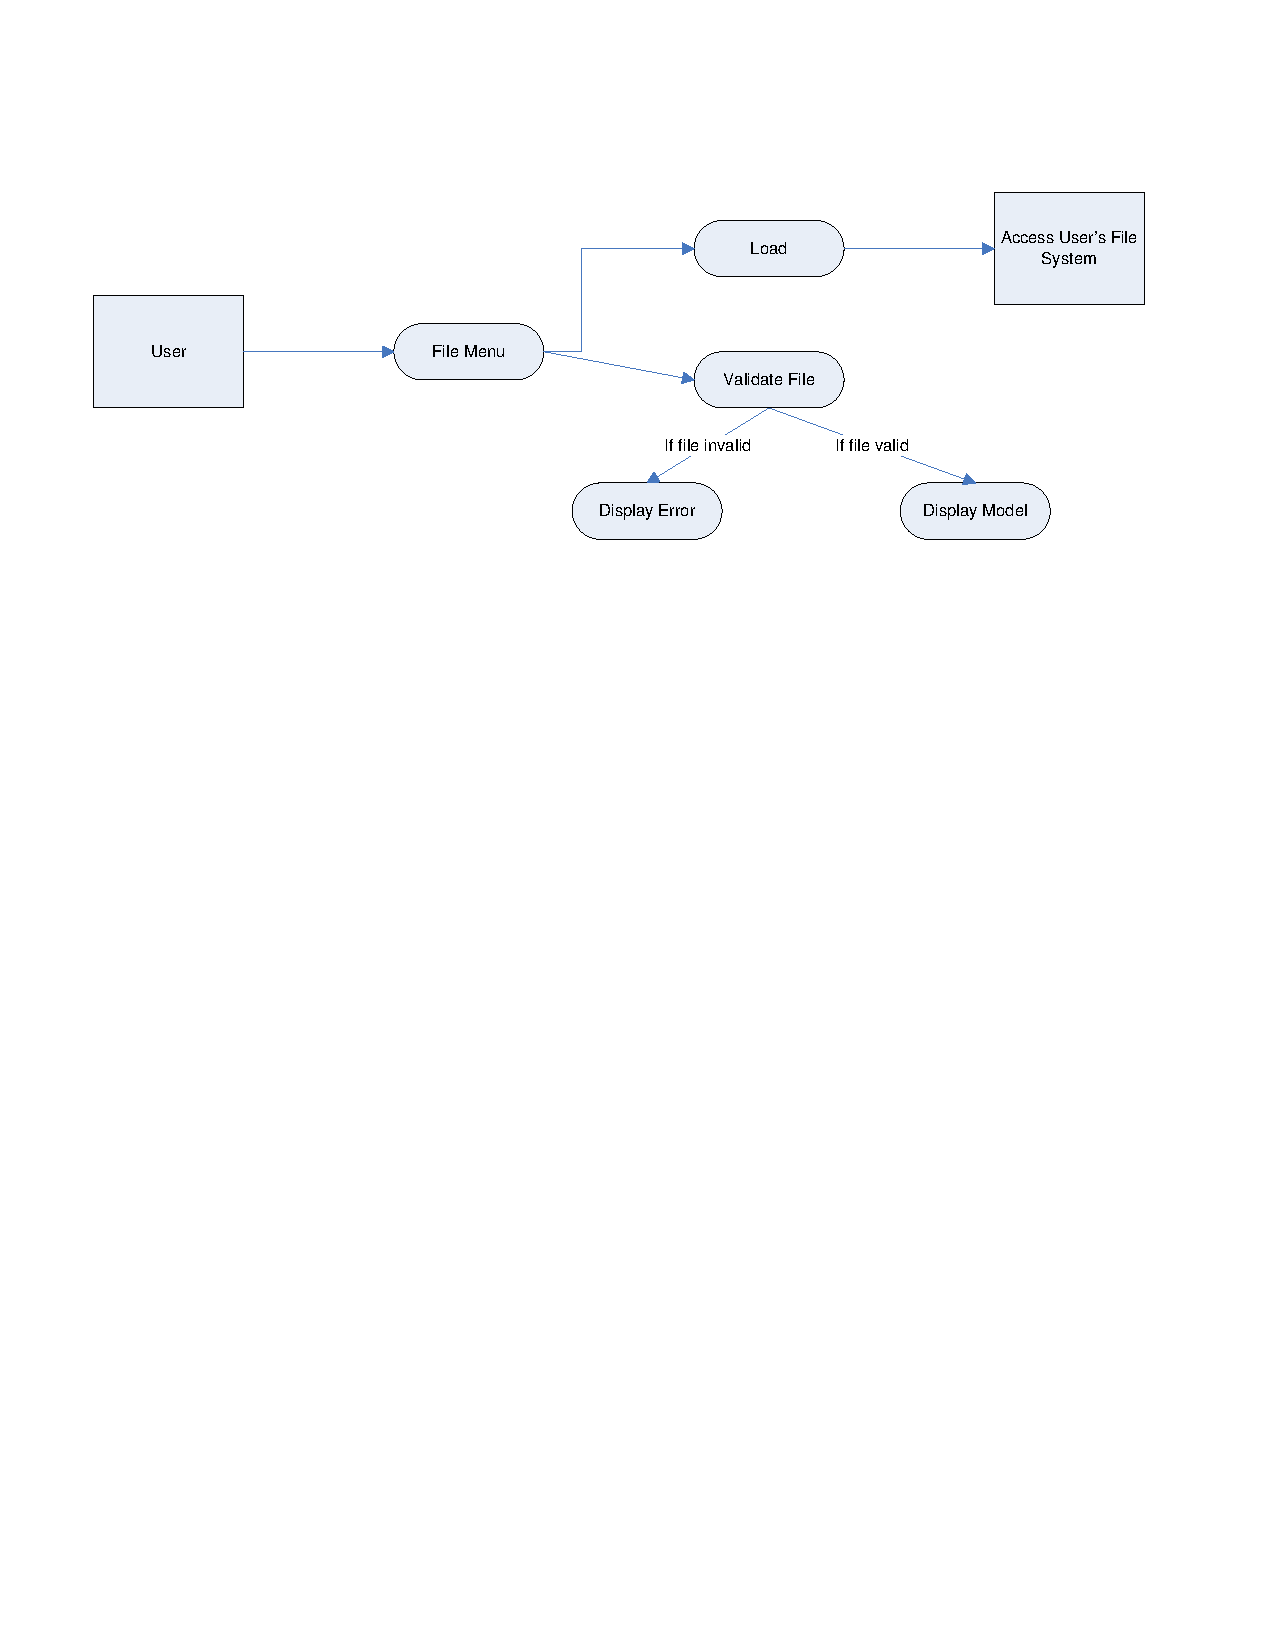
\includegraphics[width=\textwidth]{./diagrams/load}
\caption{Loading Models}
\end{figure}
\subsection{Saving Models}
The user selects the ``Save'' or ``Save As...'' menu item. If the ``Save'' menu item is selected, the model is saved to the same file in the previously selected format. If the ``Save As...'' menu item is selected, the user must enter a file name and may optionally choose the file location and format. The default format is the PhysioMist XML format. If the user selects the ``Save'' menu item for an unsaved model, the ``Save As...'' dialog is presented.
\begin{figure}[!htb]
\centering
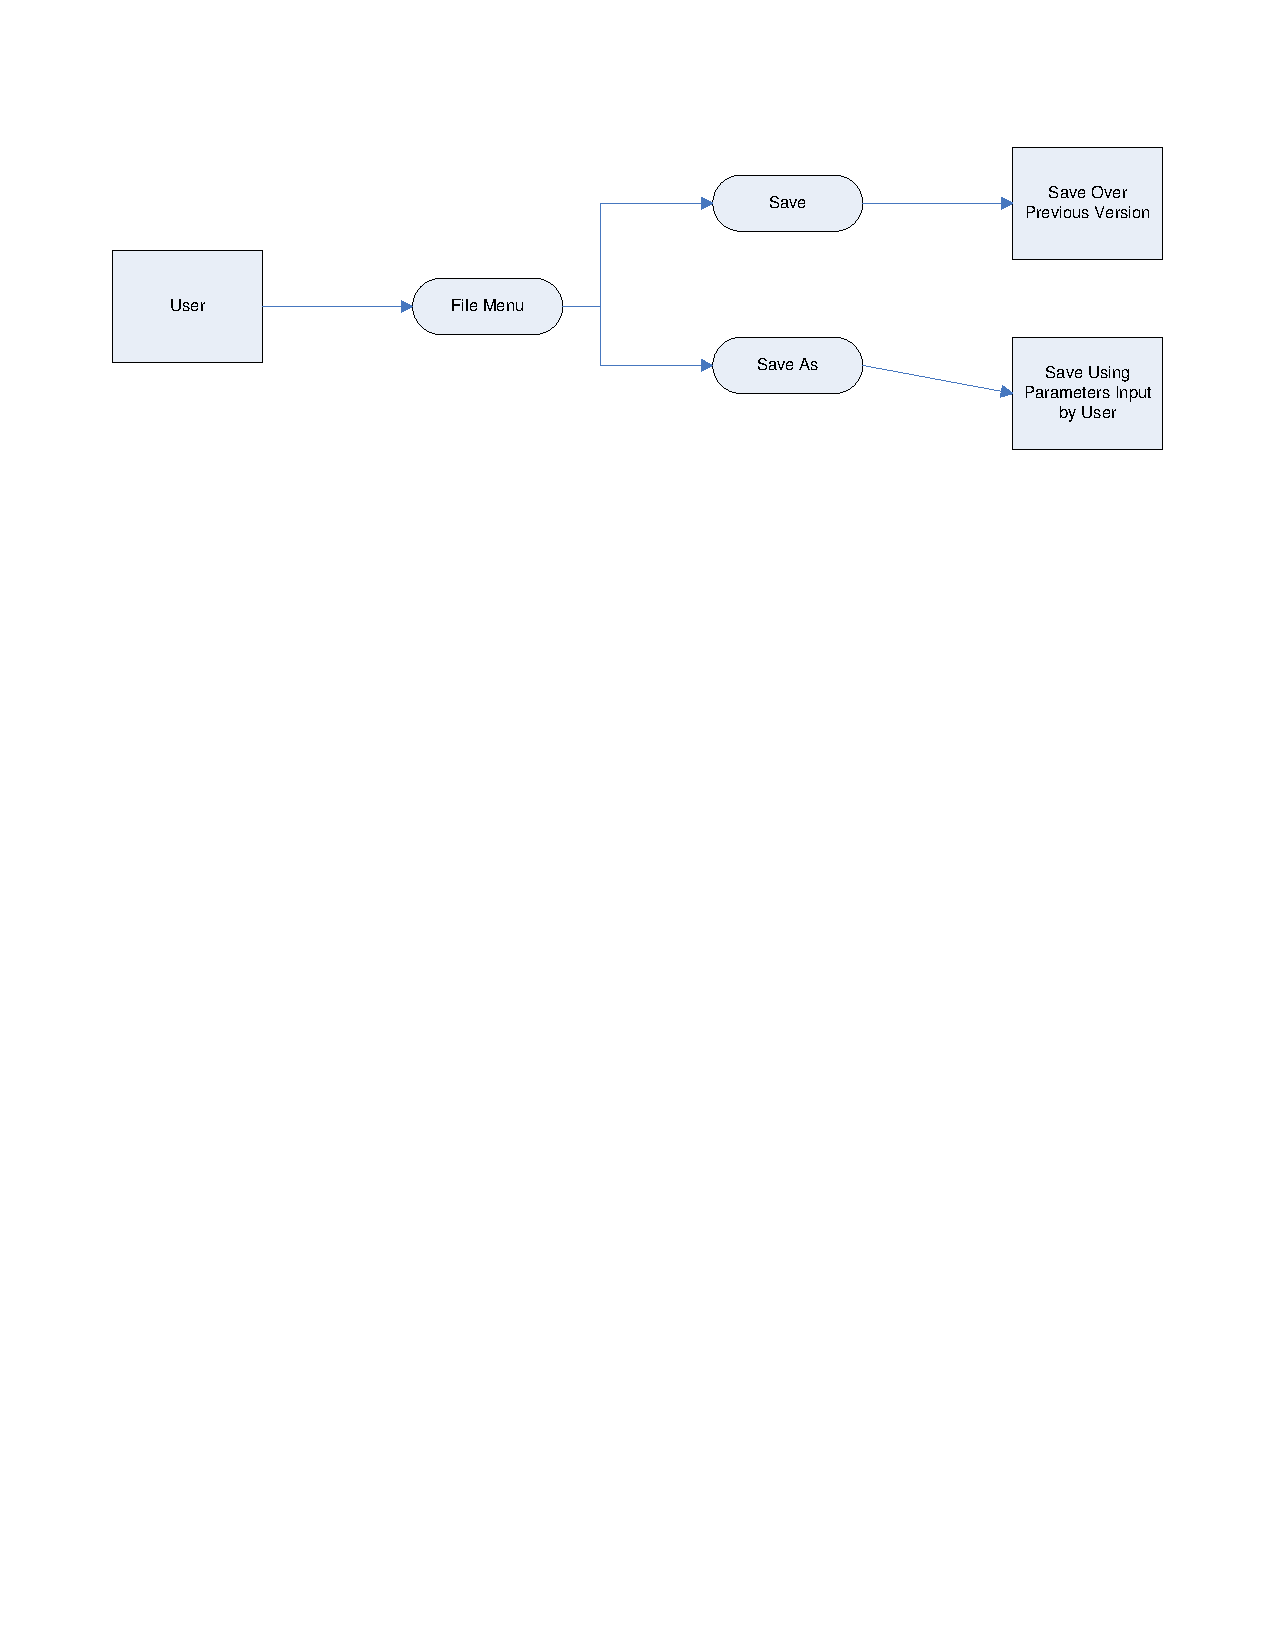
\includegraphics[width=\textwidth]{./diagrams/save}
\caption{Saving Models}
\end{figure}
\subsection{Editing Models}
\subsubsection{Adding Variables}
The user clicks the ``New'' button for the variable or parameter table. A dialog box with fields for the name, formula, value, units, anatomical structure, and description is displayed. The user enters the relevant data, the input is validated, and the new item is added to the appropriate table. Only the name, formula, and value fields are required.
\begin{figure}[!htb]
\centering
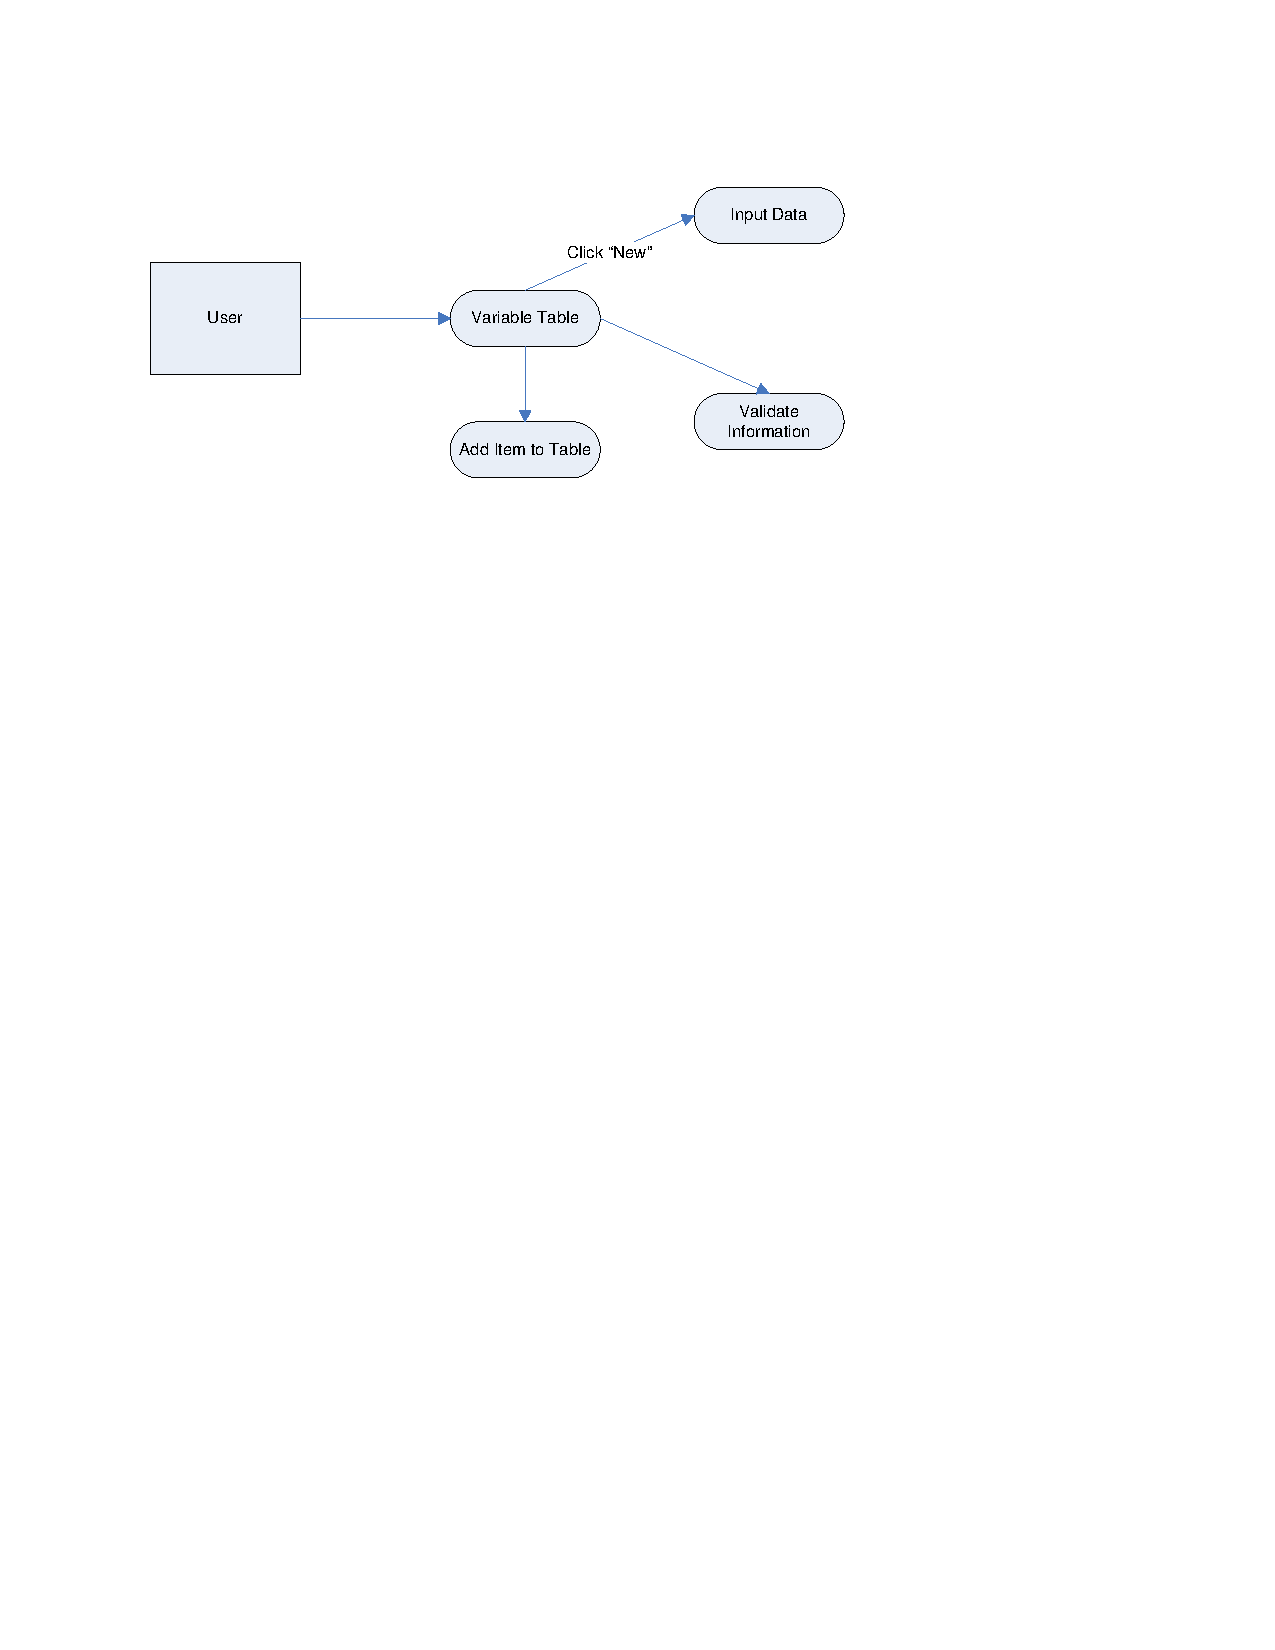
\includegraphics[width=\textwidth]{./diagrams/new-var}
\caption{Adding Variables}
\end{figure}
\subsubsection{Deleting Variables}
The user selects an item in the variable or parameter table and clicks the ``Delete'' button. The item is deleted from the model.
\begin{figure}[!htb]
\centering
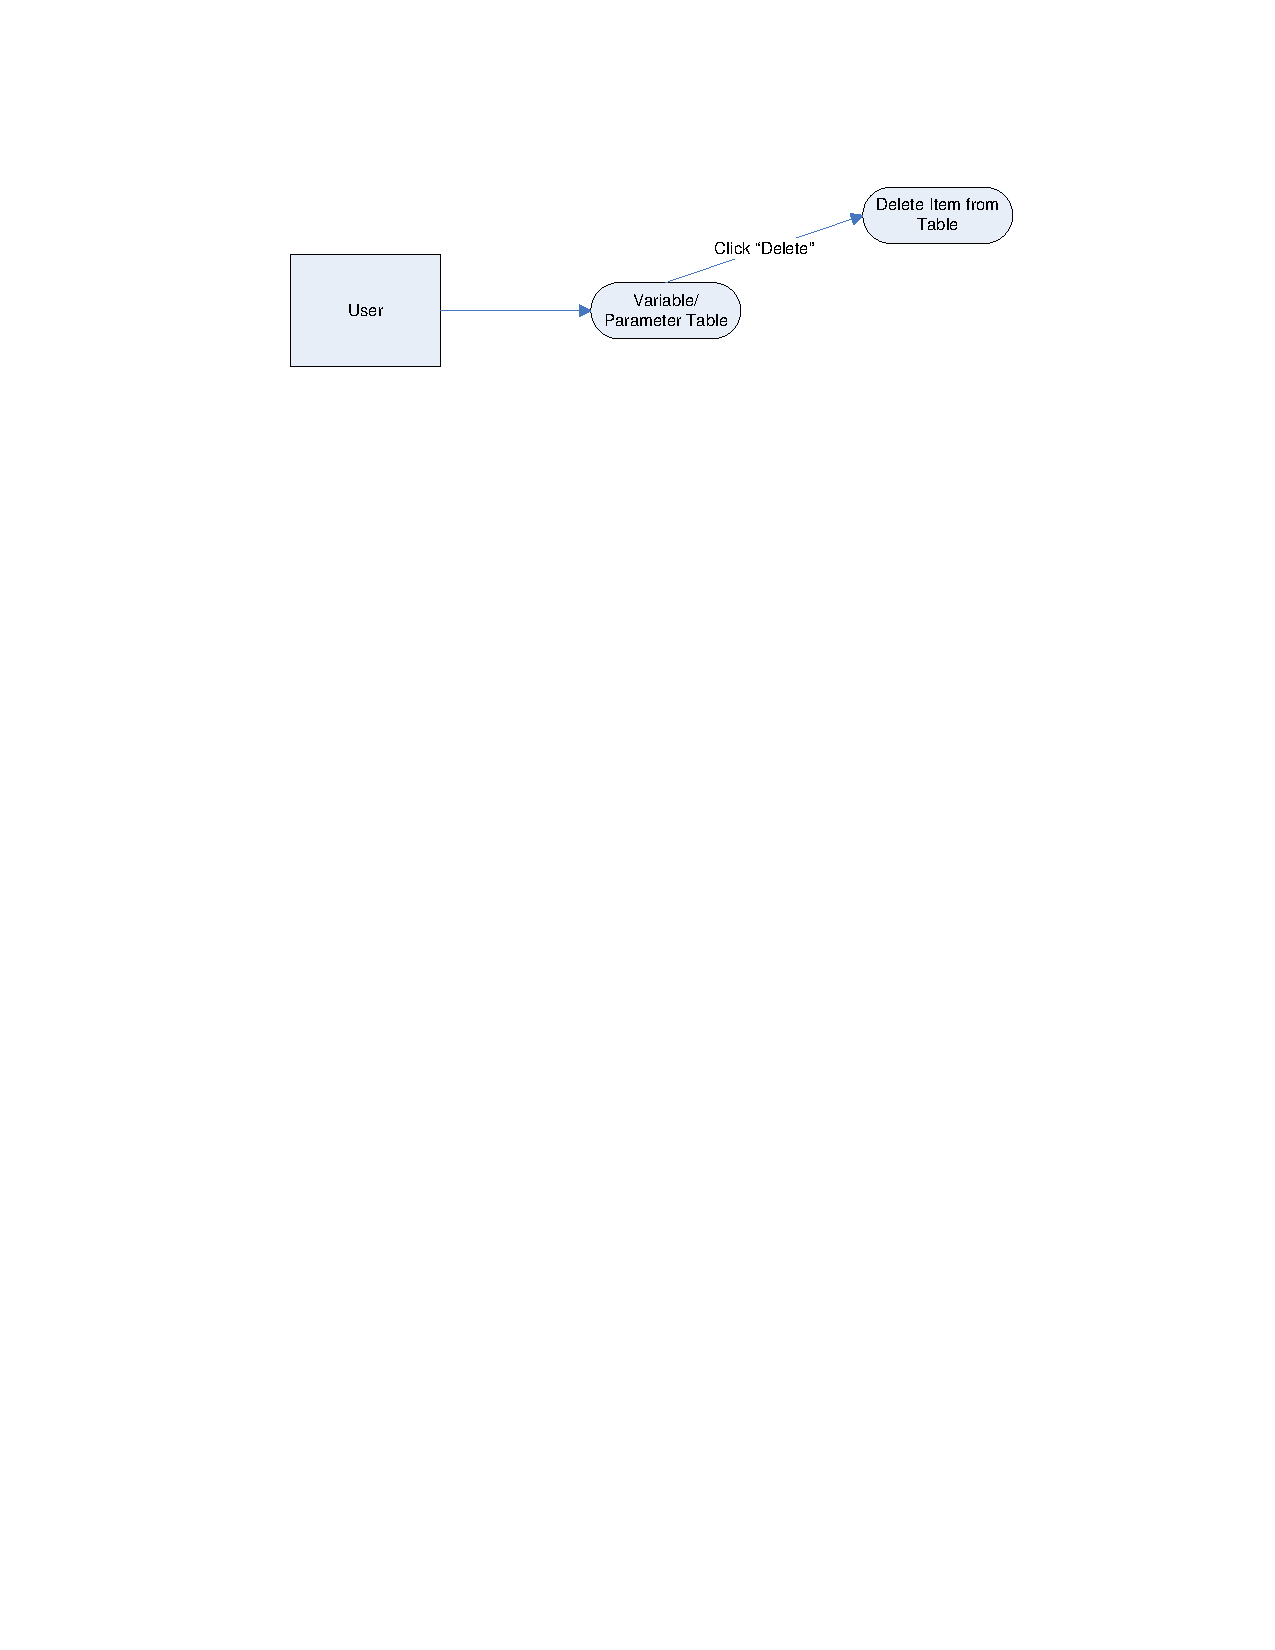
\includegraphics[width=\textwidth]{./diagrams/delete}
\caption{Deleting Variables}
\end{figure}
\subsubsection{Modifying Variables}
The user selects an item in the variable or parameter table and clicks the ``Edit'' button. A dialog box as described above is displayed with the appropriate information in the relevant fields. The user modifies the data as needed, the input is validated, and the item is modified.
\begin{figure}[!htb]
\centering
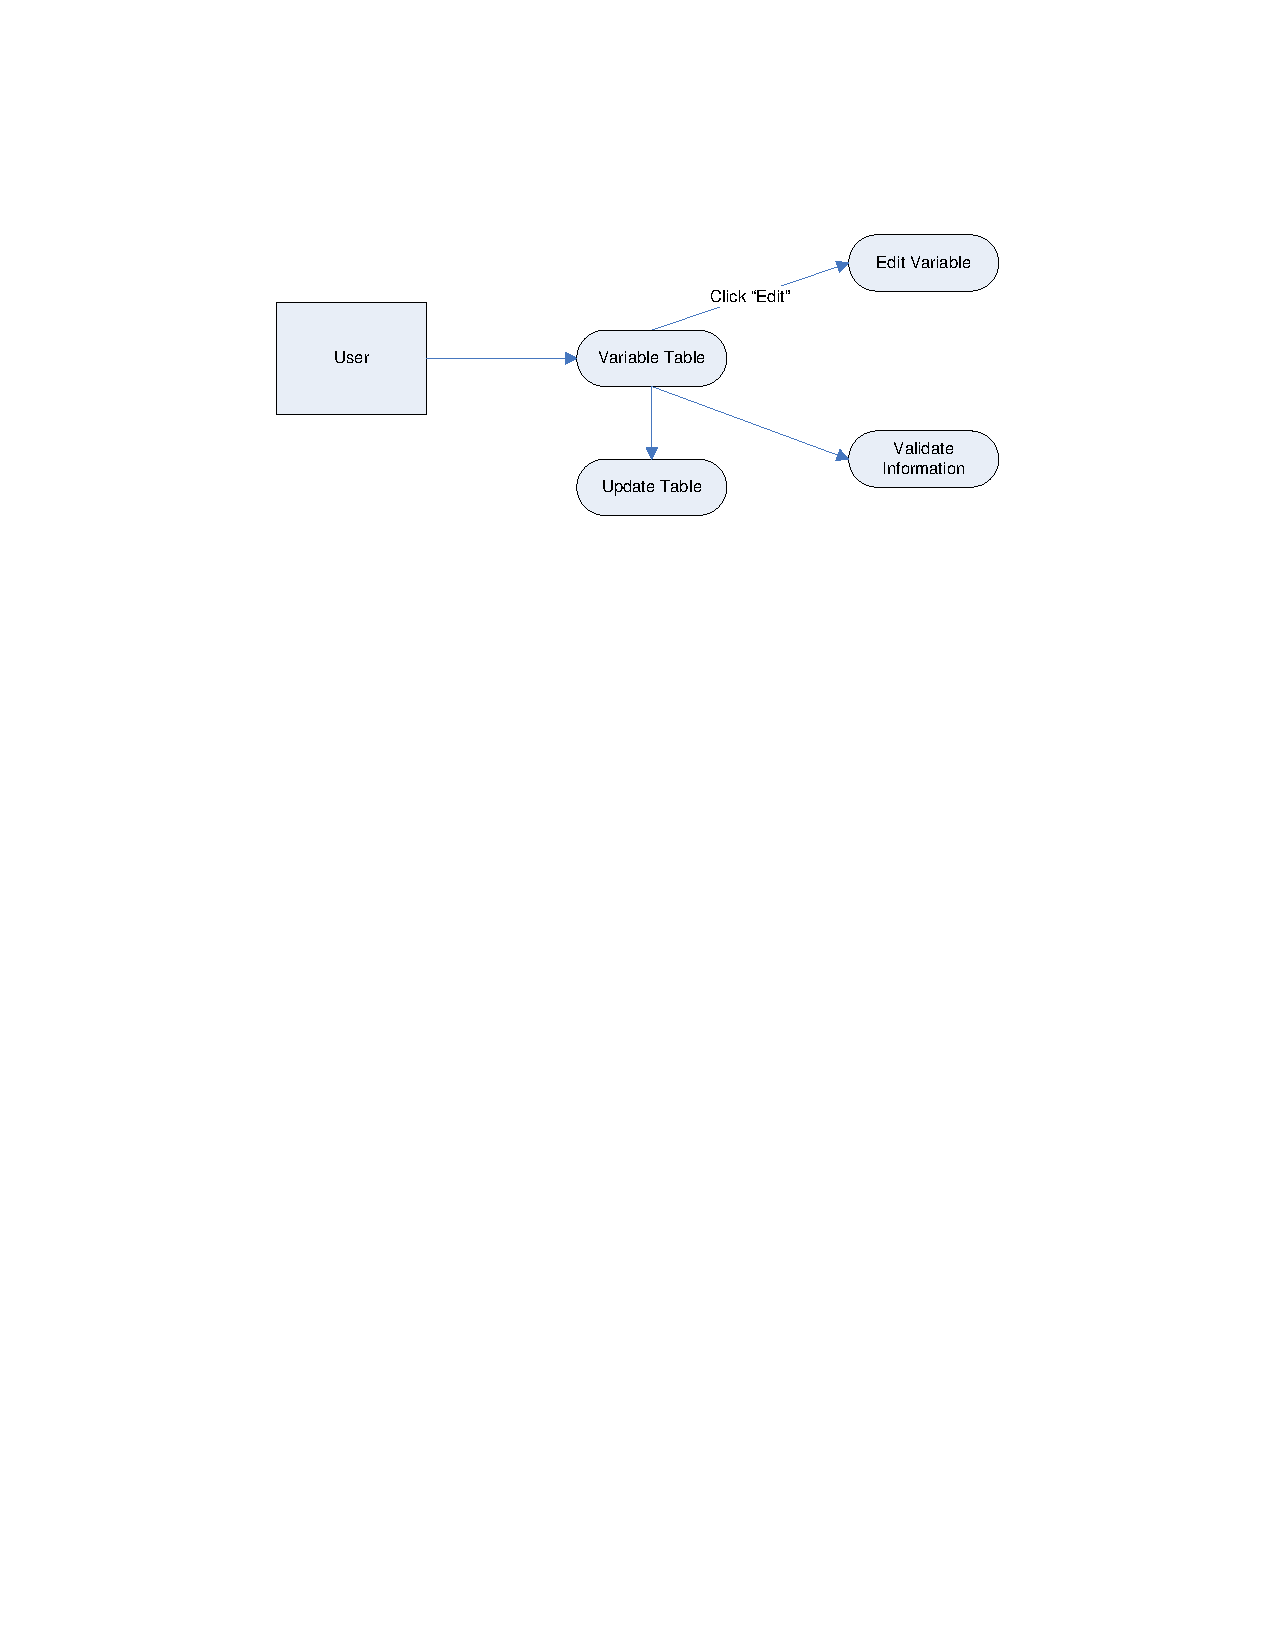
\includegraphics[width=\textwidth]{./diagrams/edit-var}
\caption{Modifying Variables}
\end{figure}
\subsubsection{Associating Anatomical Information}
When the user is editing an item in the model, the user selects an anatomical structure in the Anatomical Ontology treeview and clicks the ``Associate Structure'' button. The structure is added to the item or replaces the previous structure.
\begin{figure}[!htb]
\centering
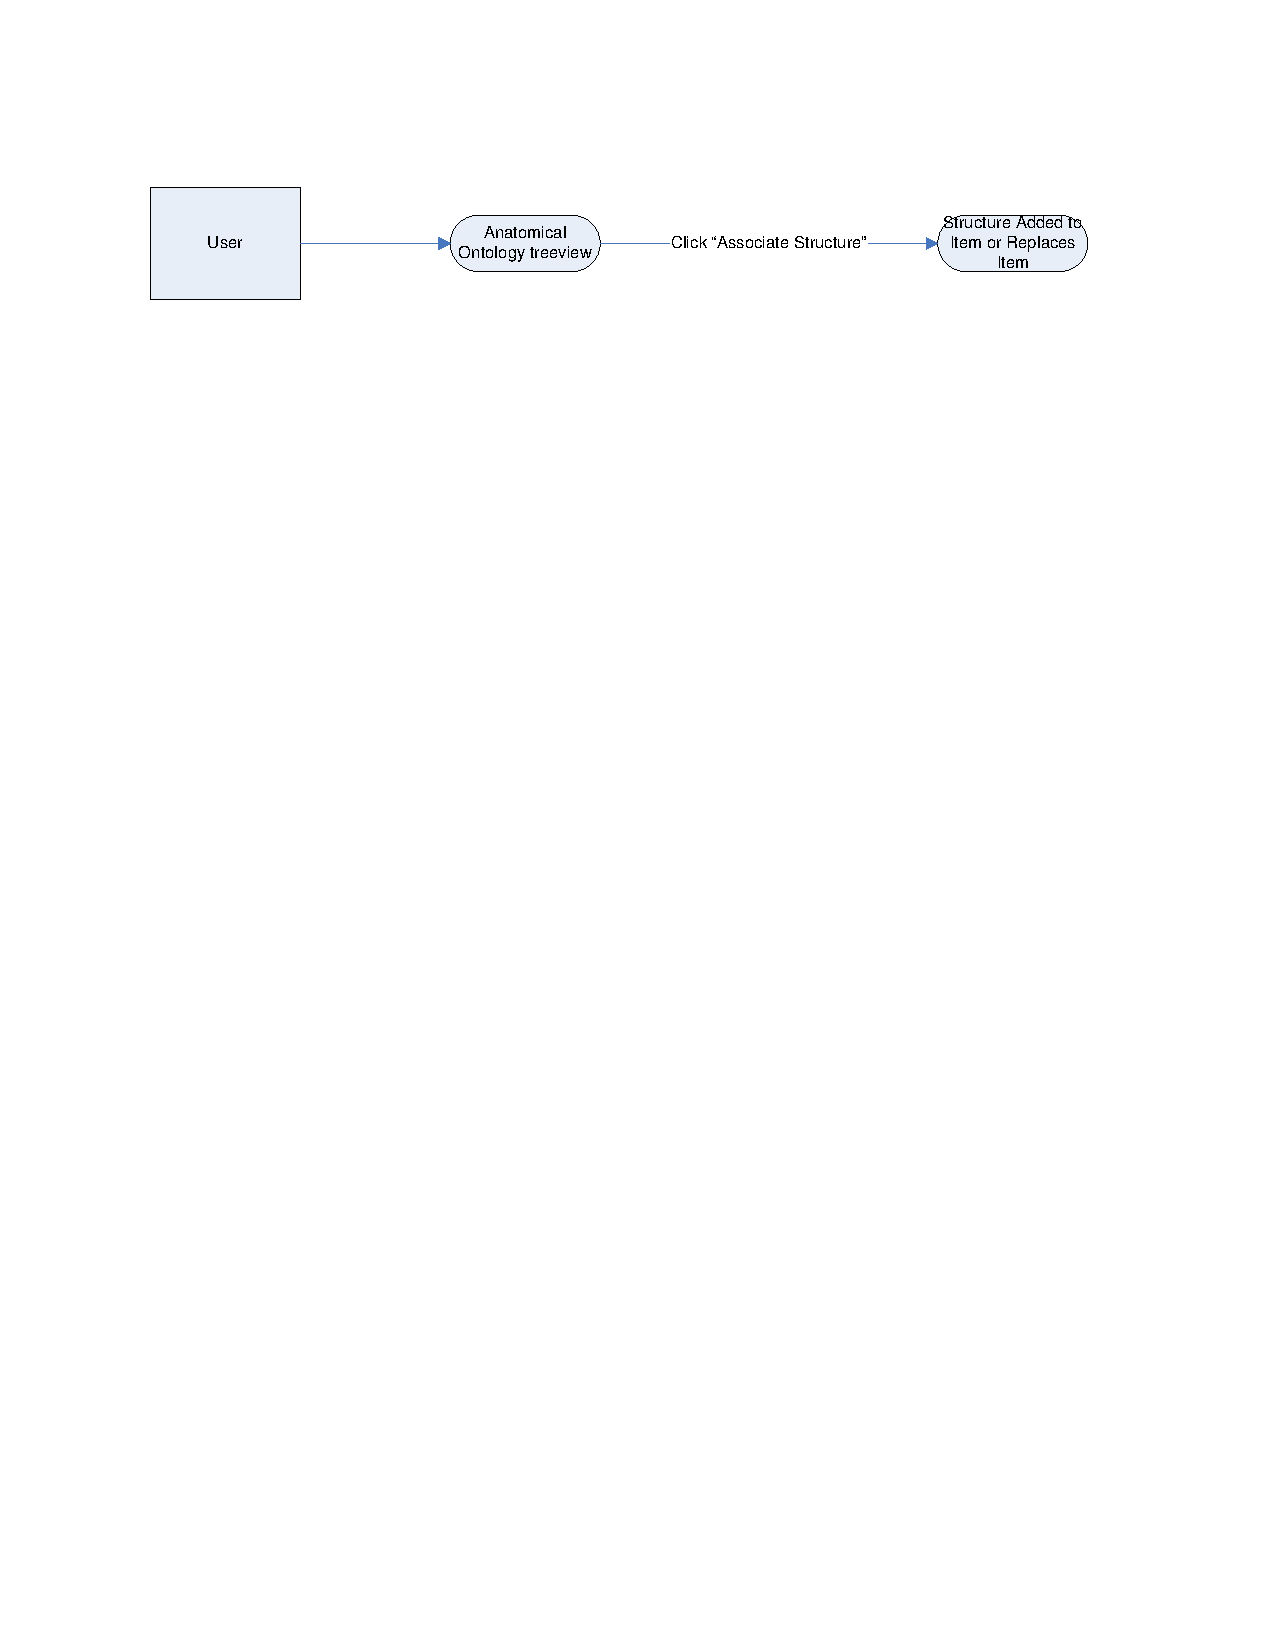
\includegraphics[width=\textwidth]{./diagrams/anatomy}
\caption{Associating Anatomical Information}
\end{figure}
\subsection{Model Integration}
This section is only concerned with integrating two models. The ability to integrate more than two models at a time may be a feature added in a future release.
\subsubsection{One-to-One Integration}
The user selects two models, which are loaded by the software as described above. The models will be referred to as $A$ and $B$ for clarity. The user then selects an item from each model ($A.x$ and $B.y$) and defines the relationship between them where $A.x$ acts as an input to $B.y$. This can be expressed mathematically as $F(A.x) = B.y$. Note that $A.x$ may be a variable or parameter, but $B.y$ must be a variable. The operations of the integration subsystem will not be addressed within this document.
\begin{figure}[!htb]
\centering
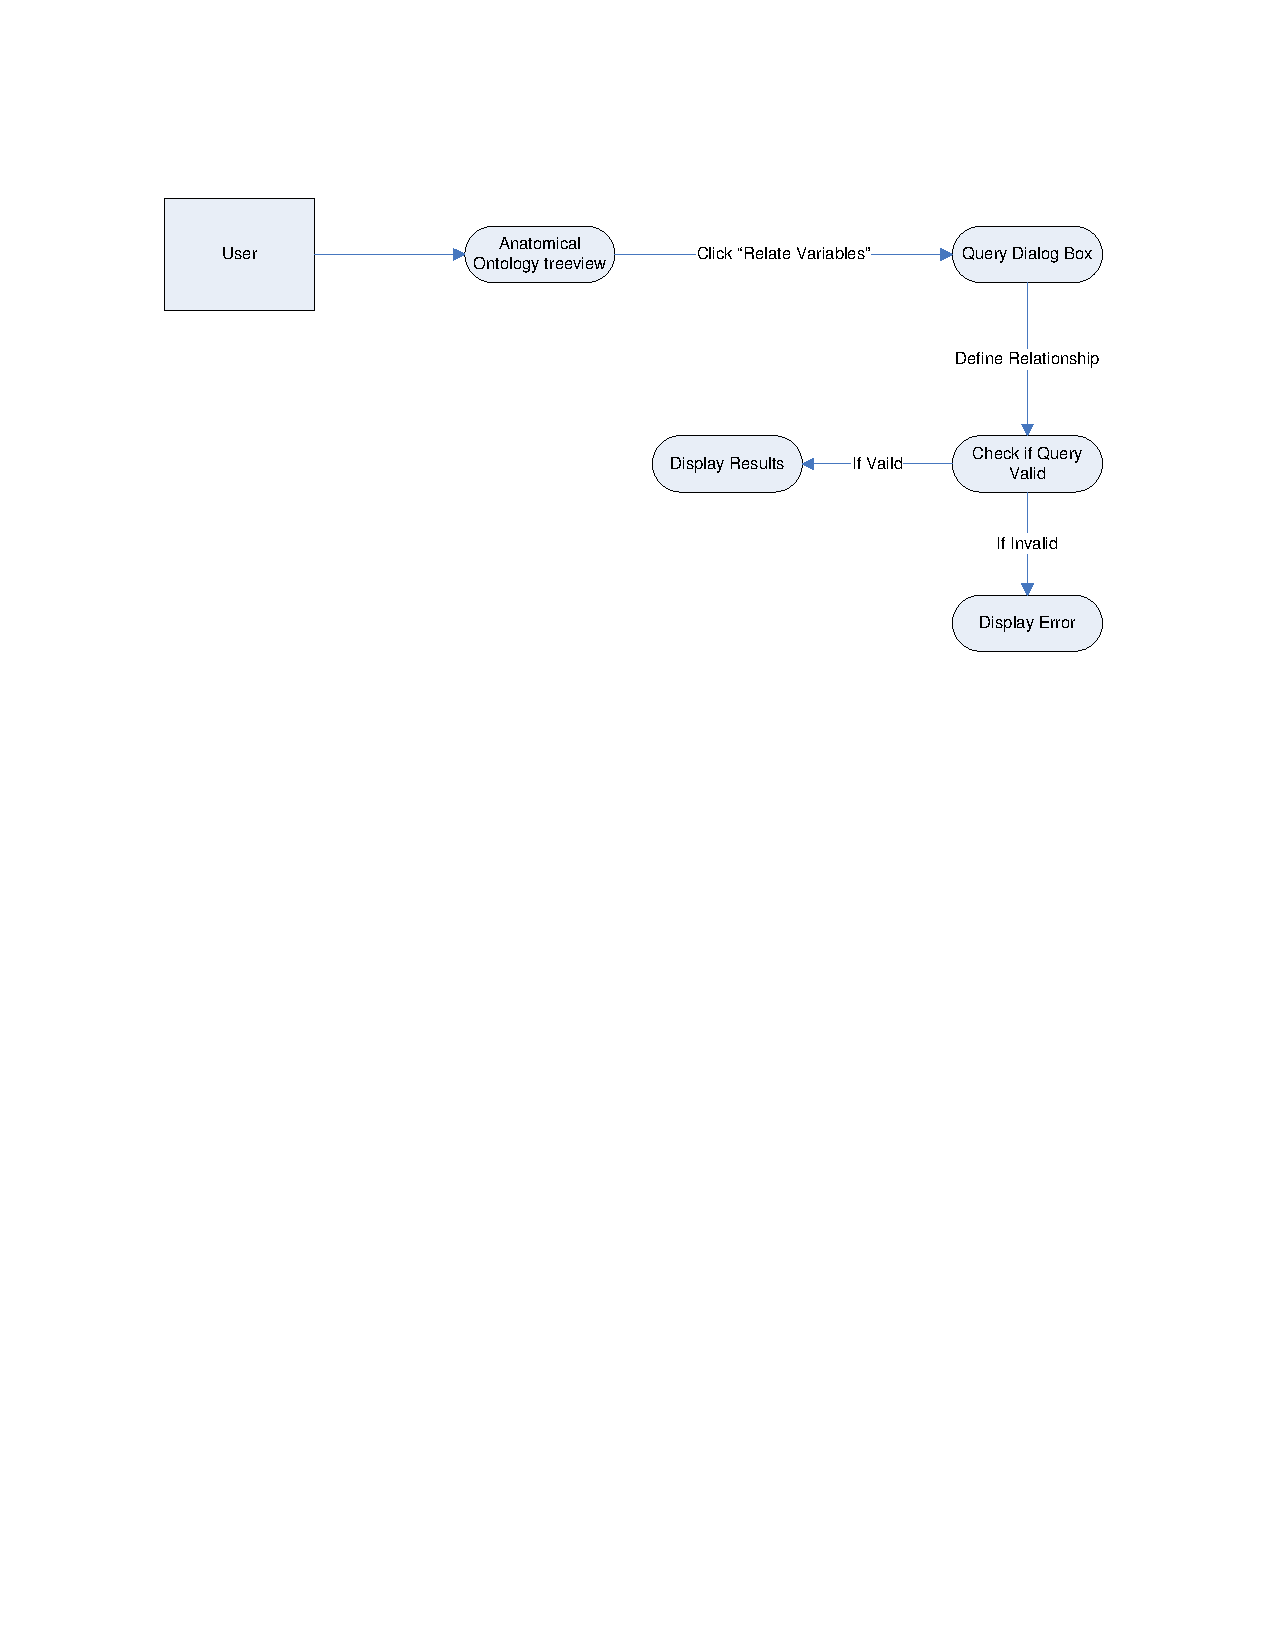
\includegraphics[width=\textwidth]{./diagrams/relate-vars}
\caption{One-to-One Variable Integration}
\end{figure}
\subsubsection{One-to-Many Integration}
This is very similar to one-to-one integration. If a relationship between $A.x$ and $B.y$ exists, the user is not restricted from defining a relationship with $A.x$ as input and $B.z$ as output. If $A.x$ is a variable and $B.w$ is not dependant upon $A.x$, the user may also define a relationship with $B.w$ as input to $A.x$. Circular relationships are handled by the underlying integration subsystem.
\subsubsection{Many-to-One Integration}
This feature may be added in a future release.
\subsection{Anatomical Queries}
\todo{list/explain the different relationship types}
\subsubsection{Structure-based Queries}
The user selects a structure in the Anatomical Ontology treeview and clicks the ``Related Structures'' menu item. The user then selects the type of relationship from the query dialog box. The software displays the results of the query (structures with the appropriate relationship to the selected structure) or an error if the relationship type is not applicable for the selected structure.
\begin{figure}[!htb]
\centering
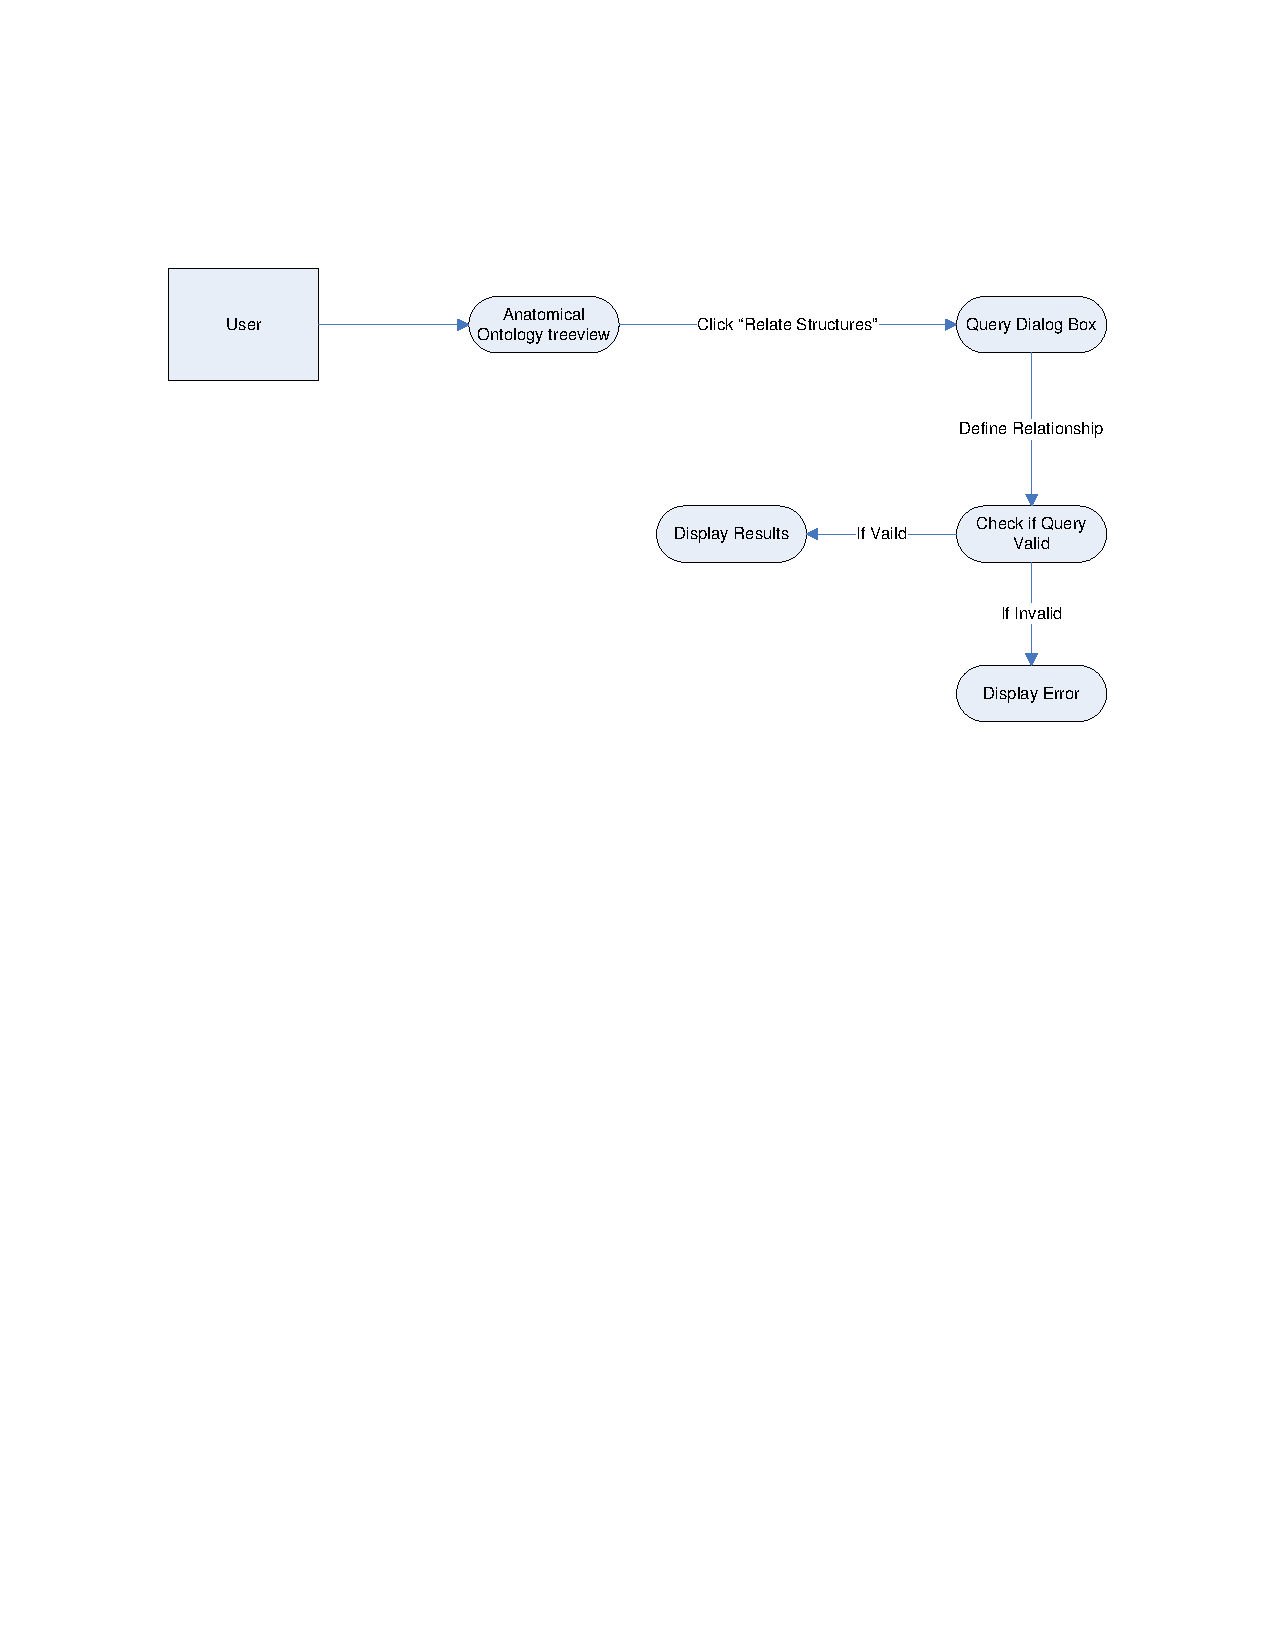
\includegraphics[width=\textwidth]{./diagrams/query-str}
\caption{Structure-based Queries}
\end{figure}
\subsubsection{Variable-based Queries}
While integrating models, the user selects a variable/parameter from one model and clicks the ``Related Variables'' menu item. The user then selects the type of relationship from the query dialog box. The software displays the results of the query (variables/parameters from both models that are associated with structures that have the appropriate relationship to the selected item's associated anatomical structure) or an error if the relationship type is not applicable for the selected item's associated anatomical structure. An error is also displayed if the selected item does not have an associated anatomical structure.
\begin{figure}[!htb]
\centering
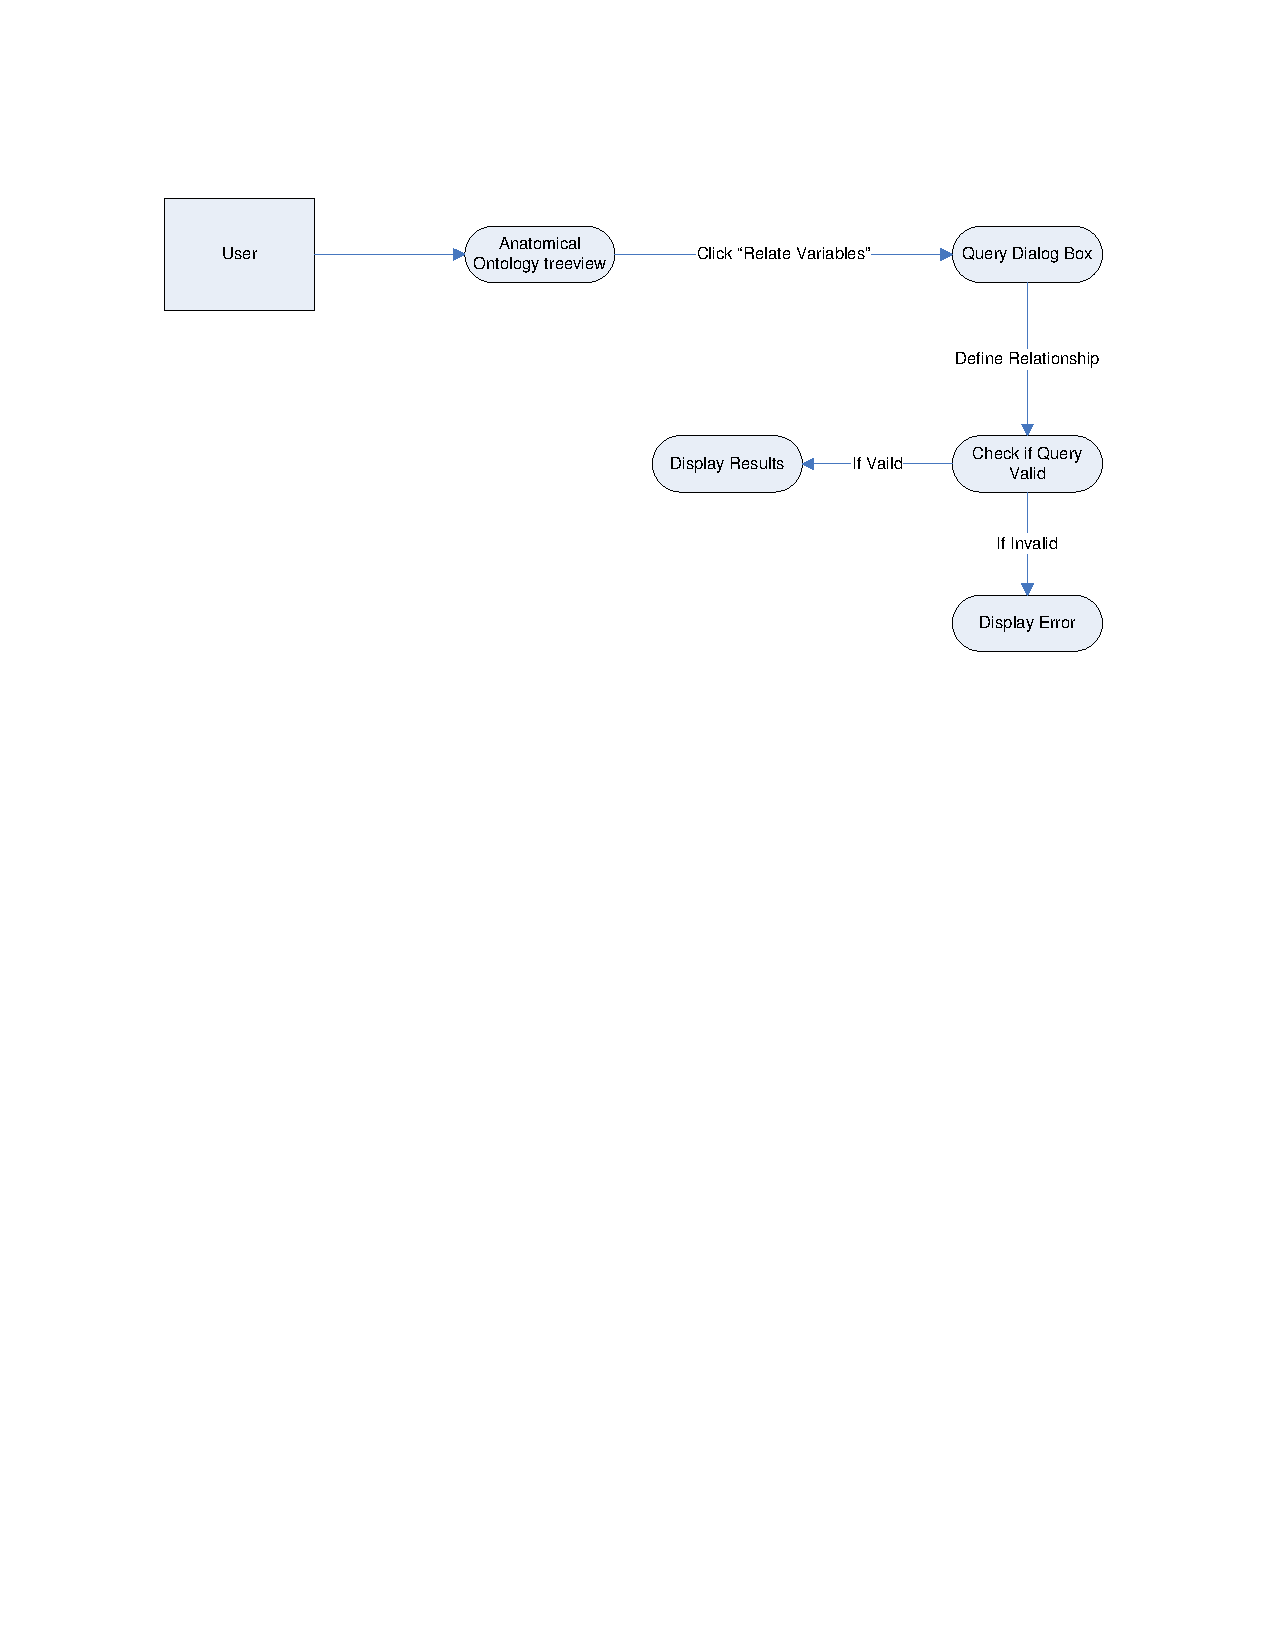
\includegraphics[width=\textwidth]{./diagrams/query-var}
\caption{Variable-based Queries}
\end{figure}

\section{Logical View}
\todo{functional requirements, object model}

\section{Process View}
The software only executes one process at a time. The software is not multithreaded.

\section{Deployment View}
Once a user has the application on his or her computer, the user's computer can run the application without interacting with any external entities.
The interactions involved in downloading the application will occur approximately as follows:
\todo{insert figure} 

\section{Implementation View}
\todo{layers and subsystems}

\section{Data View}
\todo{describe saving/loading models, the XML schema, etc}

\section{Size and Performance}
Volumes:
\newline
Although we hope that a large number of users will be interested in this application, the exact number of users does not matter since each user will have his or her own computer.  The owner of the website on which PhysioMIST is released may to need to account for excessive downloads if the application becomes very popular.\\
Performance:
\newline
The time to integrate models of average size on a one-to-one basis should be less than one hour.

\section{Quality}
The following quality factors are important to PhysioMIST.  As a result, related goals have been identified:\\
\textbf{Scalability}\\
Description:  System's reaction when user demands increase\\
Solution:  Owner of PhysioMIST's deployment website may need to allocation additional servers for download.\\
\textbf{Reliability}\\
Description:  System�s mean-time-between-failure\\
Solution: Failure is most likely to occur when integrating large datasets.  This will be handled by limiting the size of datasets.  Failure could also occur because of errors in the program which will be addressed with functional testing.\\
\textbf{Simplicity/Understandability}\\
Description: User�s ability to comprehend and utilize the system quickly\\
Solution: Organize the GUI in a logical manner and include a User�s Manual with the system\\
\textbf{Efficiency}\\
Description: System�s space demands on the user�s computer\\
Solution: Files will be saved as plain text or XML in order to minimize file size



\end{document}